\documentclass[aspectratio=169,11pt,t]{beamer}

% ---------- Style: matches Week 2 practice talk deck (navy, Palatino body, Helvetica labels) ----------
\usepackage[T1]{fontenc}
\usepackage{mathpazo}
\usepackage{helvet}
\usepackage{graphicx}
\usepackage{tikz}

\definecolor{navy}{HTML}{1F3864}
\definecolor{gold}{HTML}{F2C14E}
\definecolor{midgray}{HTML}{595959}
\definecolor{hairline}{HTML}{C8C8C8}

\setbeamertemplate{navigation symbols}{}
\setbeamertemplate{itemize items}{\textcolor{navy}{\footnotesize\textbullet}}
\setbeamercolor{normal text}{fg=black}
\setbeamercolor{structure}{fg=navy}
\setbeamerfont{normal text}{family=\rmfamily}
\usefonttheme{serif}

% section-label style headline like Week 2
\newcommand{\slidelabel}[1]{%
  {\sffamily\bfseries\fontsize{10}{13}\selectfont\color{navy}\MakeUppercase{#1}}\par
  \vspace{-6pt}\textcolor{hairline}{\rule{\textwidth}{0.5pt}}\par\vspace{8pt}}

% label-on-top stat tile: small caps label, then the big value below
\newcommand{\statlbl}[2]{%
  {\sffamily\fontsize{9}{11}\selectfont\color{midgray}\MakeUppercase{#1}}\par\vspace{6pt}
  {\sffamily\bfseries\fontsize{20}{23}\selectfont\color{navy}#2}}

\begin{document}

% ---------- Slide 1: Title ----------
\begin{frame}
  \vspace{55pt}
  {\sffamily\fontsize{8}{11}\selectfont\color{midgray}MSDS 696 DATA SCIENCE PRACTICUM II \quad\textbar\quad WEEK 3}\par\vspace{12pt}
  {\sffamily\bfseries\fontsize{25}{30}\selectfont\color{navy}Predicting U.S. Bank Undercapitalization}\par\vspace{9pt}
  {\fontsize{12.5}{17}\selectfont\itshape\color{midgray}Early Signs Before Undercapitalization}\par\vspace{14pt}
  {\sffamily\fontsize{9.5}{13}\selectfont Oussama Ennaciri \quad\textbar\quad July 2026}\par\vspace{6pt}
  \textcolor{navy}{\rule{\textwidth}{1.2pt}}
\end{frame}

% ---------- Slide 2: Undercapitalization ----------
\begin{frame}
  \slidelabel{Undercapitalization}
  \vfill
  \centering
  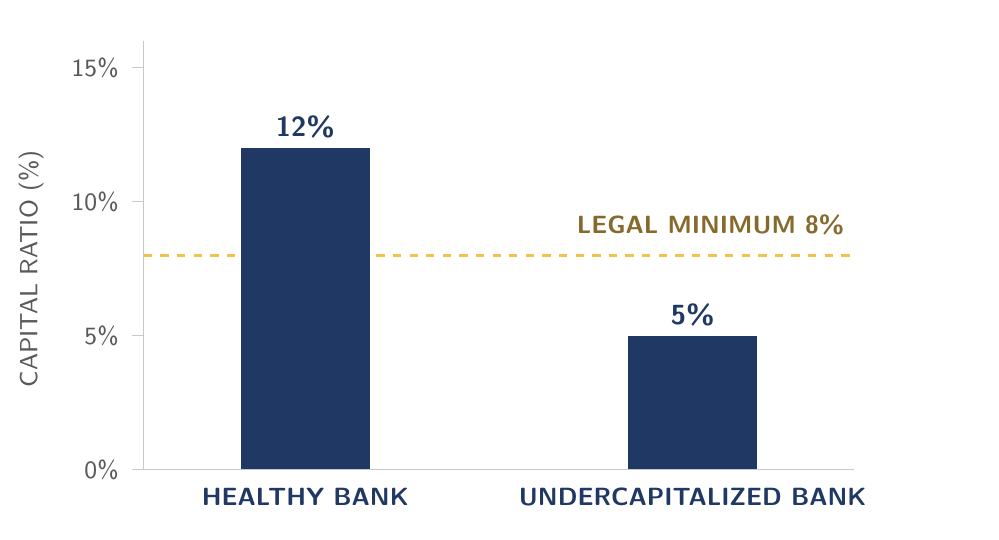
\begin{tikzpicture}[x=0.82cm,y=0.34cm]
    % bbox symmetric around bar cluster center (x=5.5)
    \useasboundingbox (-1.8,-1.6) rectangle (12.8,16.5);

    % y-axis title (rotated, on the left)
    \node[rotate=90,anchor=south] at (-1.4,7.5) {\sffamily\fontsize{9}{11}\selectfont\color{midgray}\MakeUppercase{Capital ratio (\%)}};

    % y-axis + ticks
    \draw[hairline] (0,0) -- (0,16);
    \foreach \y/\lbl in {0/0,5/5,10/10,15/15} {
      \draw[hairline] (-0.18,\y) -- (0,\y);
      \node[left] at (-0.24,\y) {\sffamily\fontsize{9}{11}\selectfont\color{midgray}\lbl\%};
    }
    % x baseline
    \draw[hairline] (0,0) -- (11,0);

    % legal minimum threshold + label
    \draw[gold,very thick,dashed] (0,8) -- (11,8);
    \node[anchor=south east] at (11,8.4) {\sffamily\bfseries\fontsize{9}{11}\selectfont\color{gold!55!black}\MakeUppercase{Legal minimum 8\%}};

    % Healthy bank
    \fill[navy] (1.5,0) rectangle (3.5,12);
    \node[above] at (2.5,12) {\sffamily\bfseries\fontsize{10}{12}\selectfont\color{navy}12\%};
    \node[below] at (2.5,-0.35) {\sffamily\bfseries\fontsize{9.5}{11}\selectfont\color{navy}\MakeUppercase{Healthy bank}};

    % Undercapitalized bank
    \fill[navy] (7.5,0) rectangle (9.5,5);
    \node[above] at (8.5,5) {\sffamily\bfseries\fontsize{10}{12}\selectfont\color{navy}5\%};
    \node[below] at (8.5,-0.35) {\sffamily\bfseries\fontsize{9.5}{11}\selectfont\color{navy}\MakeUppercase{Undercapitalized bank}};
  \end{tikzpicture}
  \vfill
\end{frame}

% ---------- Slide 3: The finding ----------
\begin{frame}
  \slidelabel{The finding}
  \vspace{6pt}
  \centering
  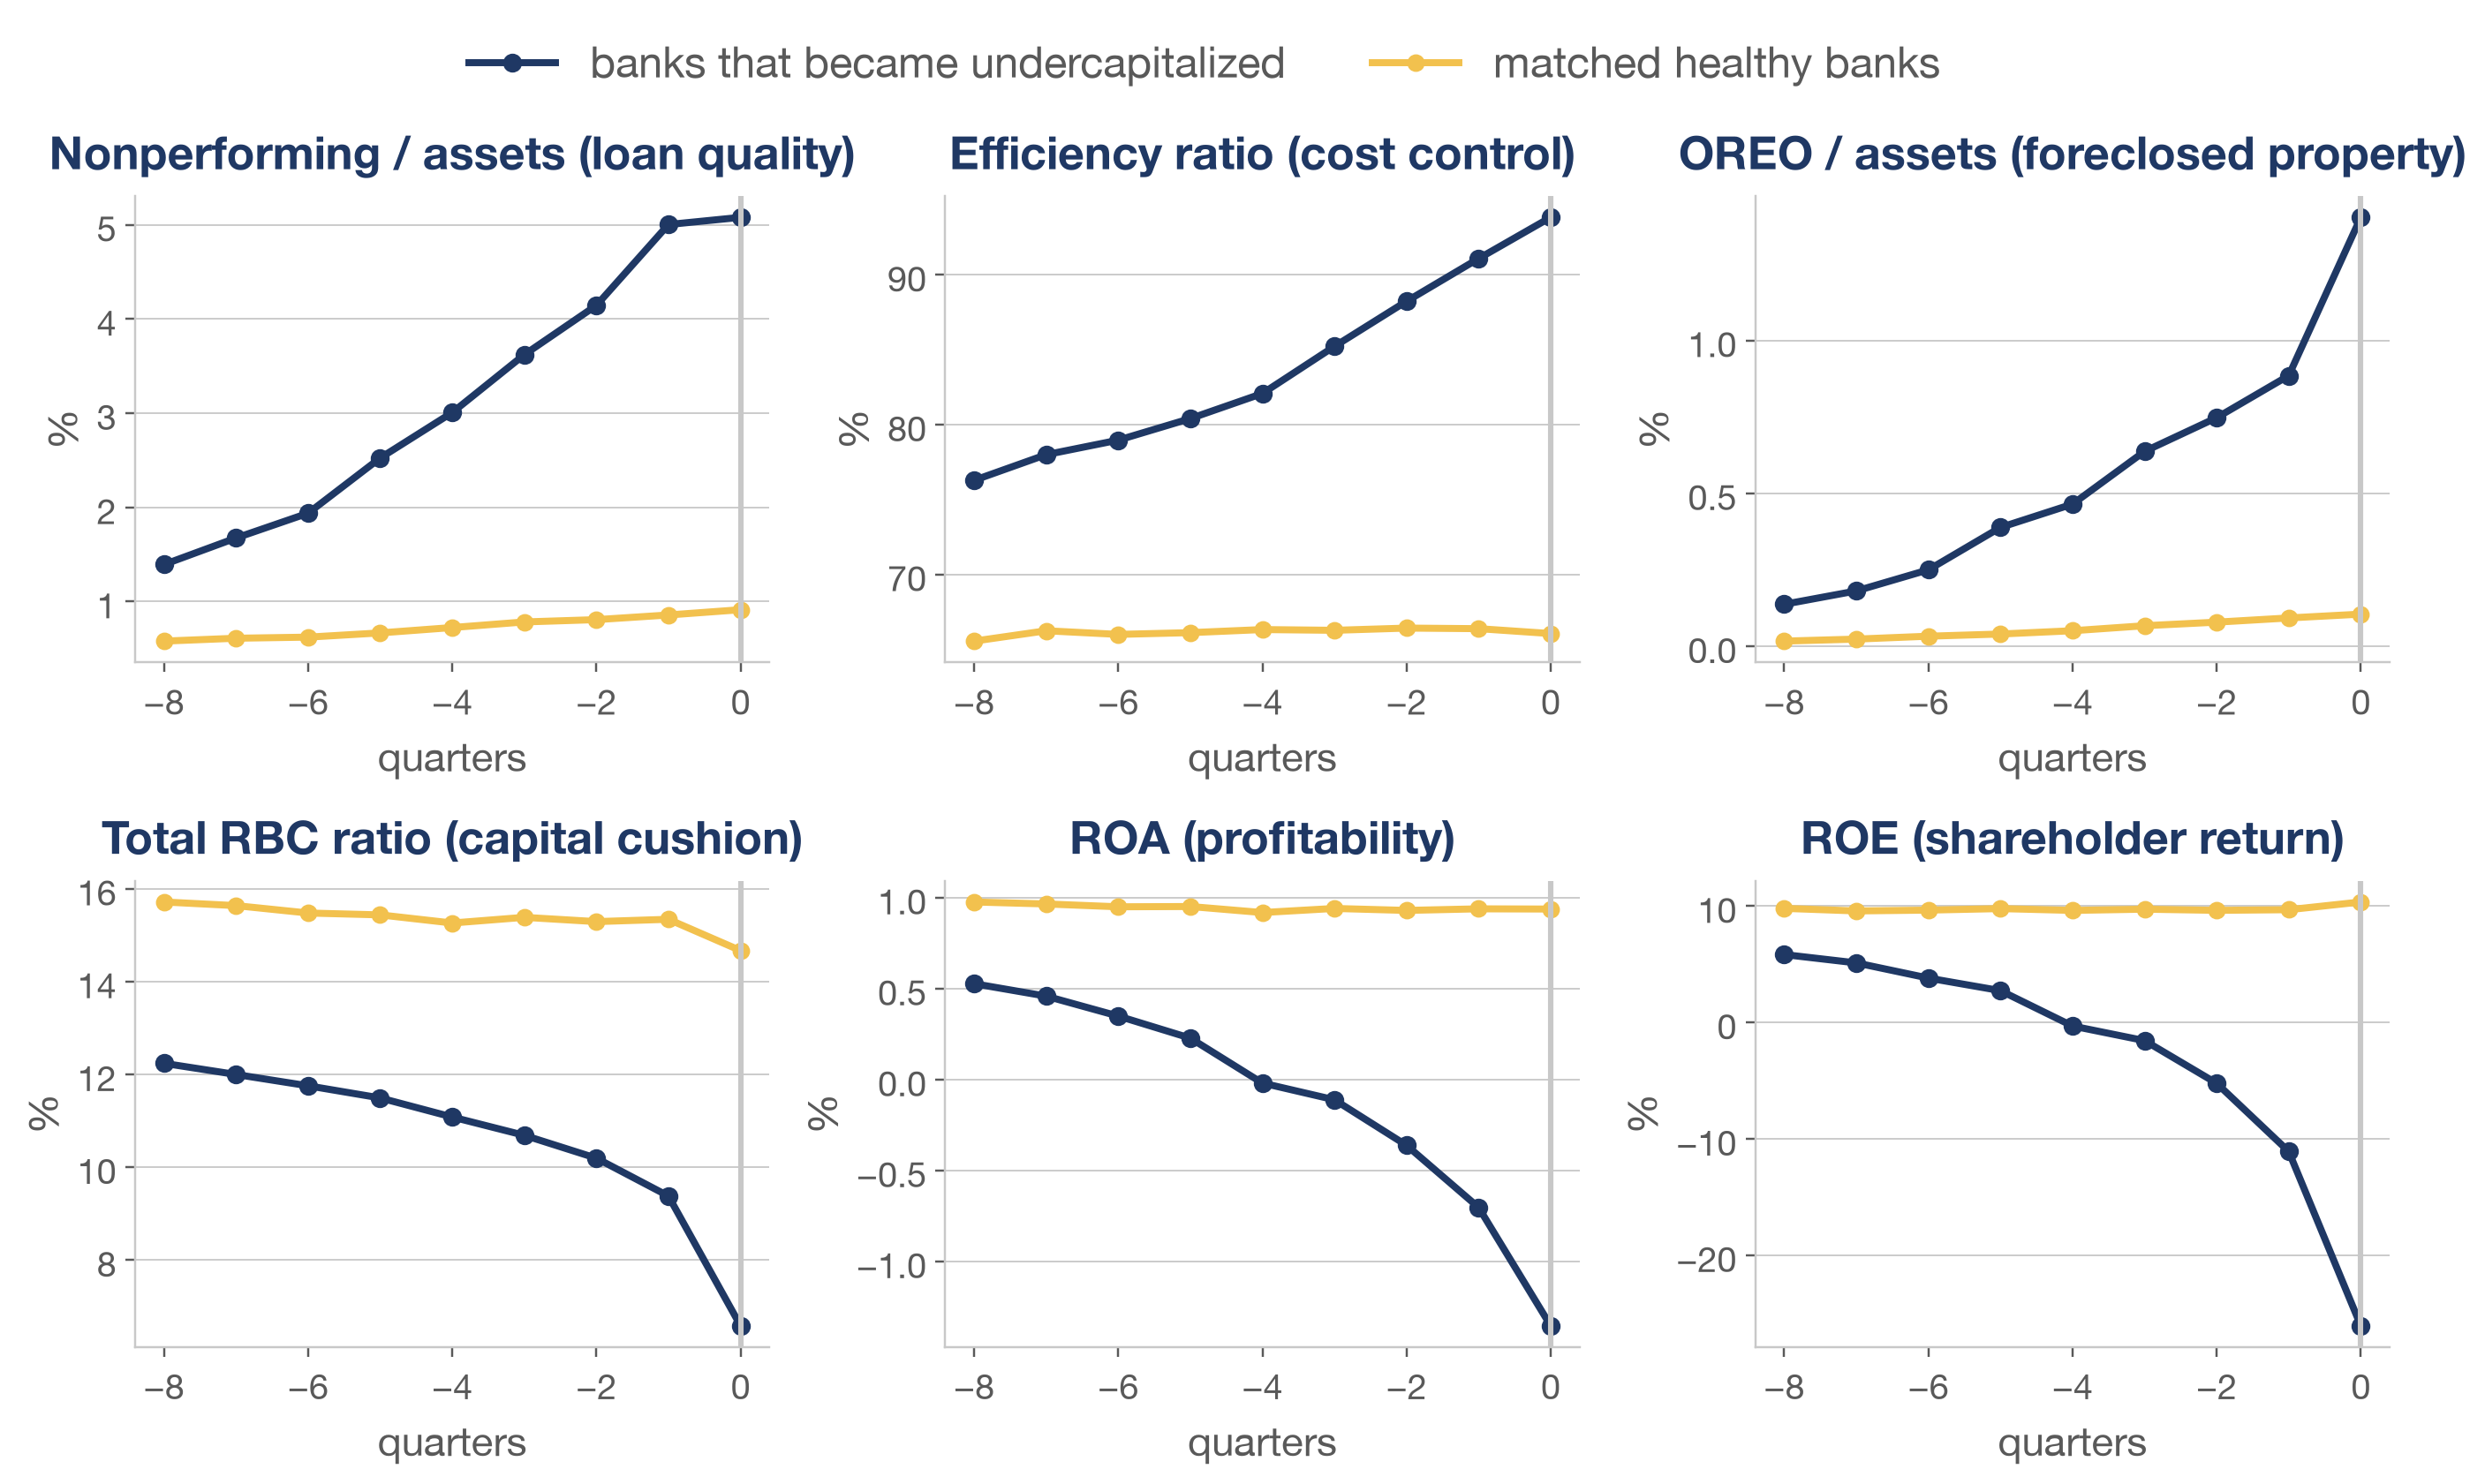
\includegraphics[width=\textwidth,height=0.80\textheight,keepaspectratio]{assets/road_to_trouble.png}
\end{frame}

\end{document}
